\documentclass{article}
\usepackage{graphicx} % Required for inserting images
\usepackage[margin=1in]{geometry}
\usepackage{amsmath}
\usepackage{amsthm}
\usepackage{amssymb}
\usepackage{amsfonts}
\usepackage{enumitem}
\usepackage{verbatim}
\usepackage{xcolor}

\title{Homework 2: Report}
\author{Dante Buhl}
\date{April. $29^{th}$ 2024}


\DeclareMathOperator{\cond}{cond}
\DeclareMathOperator{\vecspan}{span}

\begin{document}

\newcommand{\bs}[1]{\boldsymbol{#1}}
\newcommand{\bmp}[1]{\begin{minipage}{#1\textwidth}}
\newcommand{\emp}{\end{minipage}}
\newcommand{\R}{\mathbb{R}}
%\newcommand{\Imag}{\mathbb{I}}
\newcommand{\C}{\mathbb{C}}
\newcommand{\N}{\mathcal{N}}
\newcommand{\I}{\mathrm{I}}
\newcommand{\K}{\bs{\mathrm{K}}}
\newcommand{\m}{\bs{\mu}_*}
\newcommand{\s}{\bs{\Sigma}_*}
\newcommand{\dt}{\Delta t}
\newcommand{\tr}[1]{\text{Tr}(#1)}
\newcommand{\Tr}[1]{\text{Tr}(#1)}
\newcommand{\hl}[1]{\colorbox{yellow}{#1}}
      
\maketitle

\section*{Problem 1: Absolute Stability for AB3}
\begin{enumerate}[label=\alph*)]

  \item Determine the largest value of $\Delta t$, for which the three-step 
        Adams-Bashforth method (AB3)
    \begin{proof}
      We use the condition for absolute stability: 
      \begin{align}
        \lim_{k \to \infty} ||\bs{u}_k|| = 0
      \end{align}
      For this specific numerical method, we have the following characteristic
      polynomial for the numerical method. (Note that since the columns of $B$
      are linearly independent we have that $B$ is diagonalizable).
      \begin{align}
        \bs{u}_{k+3} = \bs{u}_{k+2} + \frac{\dt}{12}\left(23\bs{f}_{k+2} -
        16\bs{f}_{k+1} + 5\bs{f}_k\right)\\
        \bs{u}_{k+3} - \bs{u}_{k+2} = \frac{\dt}{12}\left( 23\bs{Au}_{k+2} -
        16\bs{Au}_{k+1} + 5\bs{Au}_k\right)\\
        \bs{w}_{k+3} - \bs{w}_{k+2} = \frac{\dt}{12}\Lambda\left( 23\bs{w}_{k+2} -
        16\bs{w}_{k+1} + 5\bs{w}_k\right)
      \end{align}
      From this form of the Adams Bashforth method, we have that the
      coefficients $\alpha_i$ and $\beta_i$ are as follows, 
      \begin{align}
        \bs{\alpha} = [0, 0, -1, 1], \quad \bs{\beta} = \left[ \frac{5}{12},
        -\frac{16}{12}, \frac{23}{12}, 0\right]  \\
        \sum_{i=0}^3 (\alpha_i - \dt\lambda_m\beta_i)\bs{w}_{k+i}^m = 0
      \end{align}
      At this point, bother to find the eigenvalues of the matrix A which form
      $\Lambda$. Using a matlab eigenvalue solver, we find the eigenvalues of
      $A$ to be, 
      \begin{align*}
            \lambda \approx \left[ -0.9667 \pm i 30.1255, -99.0667\right]\\
            \R(\lambda) \approx \left[ -0.9667, -99.0667\right]
      \end{align*}
      We also only consider the real part of $\lambda$ as this is what will
      contribute to the convergence/stability. At this point we have 2 equations
      to solve in order to find the requirement on $\dt$ for the absolute
      convergence. The two equations are related to the characteristic
      polynomial for the iteration process. 
      \begin{align*}
        \pi(z) = \rho(z) - \dt\lambda_i\sigma(z) = 0\\
        \rho(z) = \sum_{j=0}^{q} \alpha_j z^j, \quad 
        \sigma(z) = \sum_{j=0}^{q} \beta_j z^j \\
        \rho(z) = z^3 - z^2, \quad \sigma(z) = \frac{23z^2 - 16z + 5}{12}
      \end{align*}   
      \begin{align}
        \pi(z)=0, \implies \dt = \frac{\rho(z)}{\lambda_i \sigma(z)}
      \end{align}
      This equation now becomes a constrained optimization problem. We consider
      two constraints. First, the value of $\dt$ must be a real value. We notice
      that the equation given to solve for $\dt$ is composed of three complex
      quantities, so there is no guarantee that the obtained value for $\dt$ is
      real. Second, we notice that the eigenvalues of the system that we wish to
      be a contraction must be of absolute value less than 1. That is, $|z| <
      1$. Therefore, we have two constraints, on a 3 variable optimization
      problem. We obtain three equations. 
      \begin{align}
        z = x + iy, \quad |z| < 1 &\implies x^2 + y^2 < 1\\
        \mathbb{I}(\dt) = 0 &\implies \mathbb{I}\left(\frac{\rho(x,
        y)}{\sigma(x, y)}\right) = 0\\
        \max \R(\dt) &\implies \nabla_h \R\left(\frac{\rho(x, y)}{\sigma(x,
        y)}\right) = \vec{0}
      \end{align}
      The actual function being considered here is quite unpleasant to write
      out explicitly. So the rest of this problem will proceed by the result of
      numerical work. The easiest way to solve this problem is as it is put in
      the notes. We consider the boundary of the domain for the eigenvalue, $z$,
      that will yield a contraction. This is of course the unit circle, $z =
      e^{i\theta}$. Then, we find the region of absolute stability from
      $\frac{\rho(e^{i\theta})}{\sigma(e^{i\theta})}$ (\textbf{Fig. 1}).
      \begin{figure}[h]
        \centering
        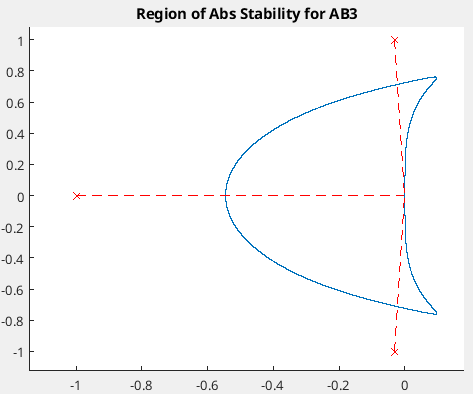
\includegraphics[width=0.5\textwidth]{1bAbsStabReg.png}
        \caption{Region of Abs. Stab. for AB3 (Blue) (inside boundary)}
      \end{figure}
      This yields a plot on the
      complex plane with eigenvalues that satisfy the problem we wish to solve.
      Then we overplot the normalized eigenvalues from our original matrix A, and draw
      lines originating from the origin to the eigenvalues of A in the complex
      plane. In order to ensure that $\dt$ is a real-valued, we must pick points
      on the region of absolute stability which are colinear with the
      eigenvalues of $A$. Then we determine the maximum $\dt$ by the ratio
      between the distance from the eigenvalue to the origin and the distance
      from the point colinear on the boundary of the region of absolute
      stability to the origin. This is then our $\dt$. We find for this problem,
      that the eigenvalue, $\lambda = -99.0667$ is furthest from the region of
      absolute stability, and appropriate $\dt$ for this eigenvalue is very
      close to $\dt = 0.00550593$. 
    \end{proof}
  \item See \textbf{Fig. 1}.

  \item We can plot the results of AB3 with three values of $\dt$. We have $\dt
  \in [10^{-4}, \dt^* - 10^{-4}, \dt^* + 10^{-4}]$, where $\dt^* = 0.0055$ (we
  only consider up to 4 decimal digits since we perturb it by $10^{-4}$). The
  results can be seen in figure 2. Evidently, above the critical $\dt$ the
  numerical method diverges and doesn't resemble that of the other two plots.
  This demonstrates the concept of absolute stability and we can see its import
  on numerical methods for ODEs and PDEs. 

  \begin{figure}
    \centering
    \begin{minipage}{0.48\textwidth}
        \centering
        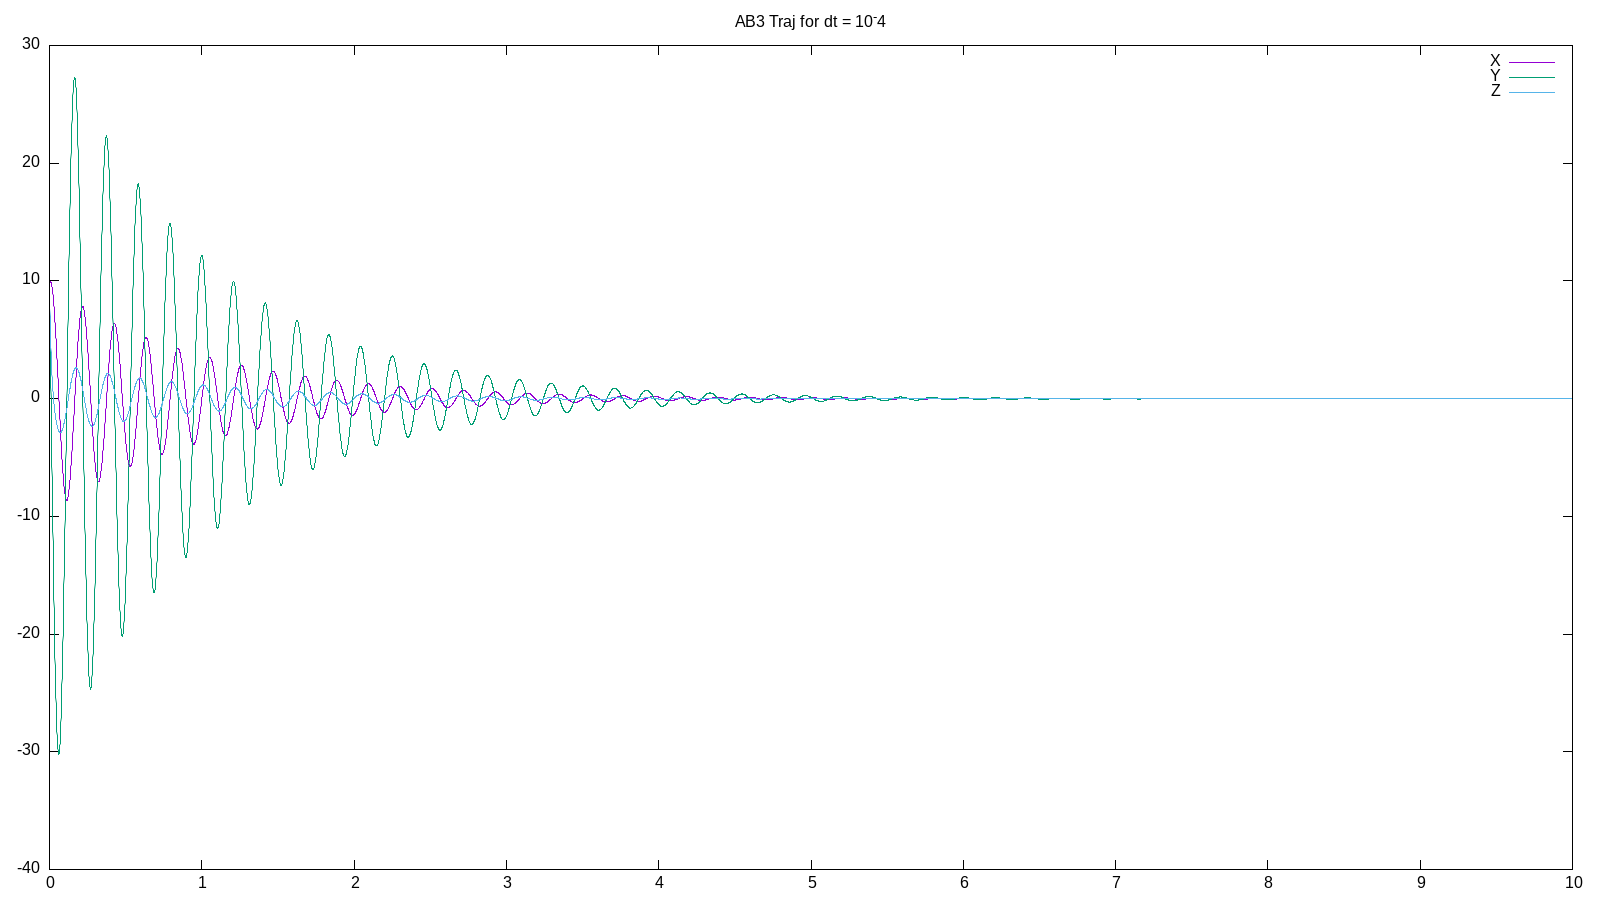
\includegraphics[width=1\textwidth]{1cdt=10-4.png}
    \end{minipage}
    \begin{minipage}{0.48\textwidth}
        \centering
        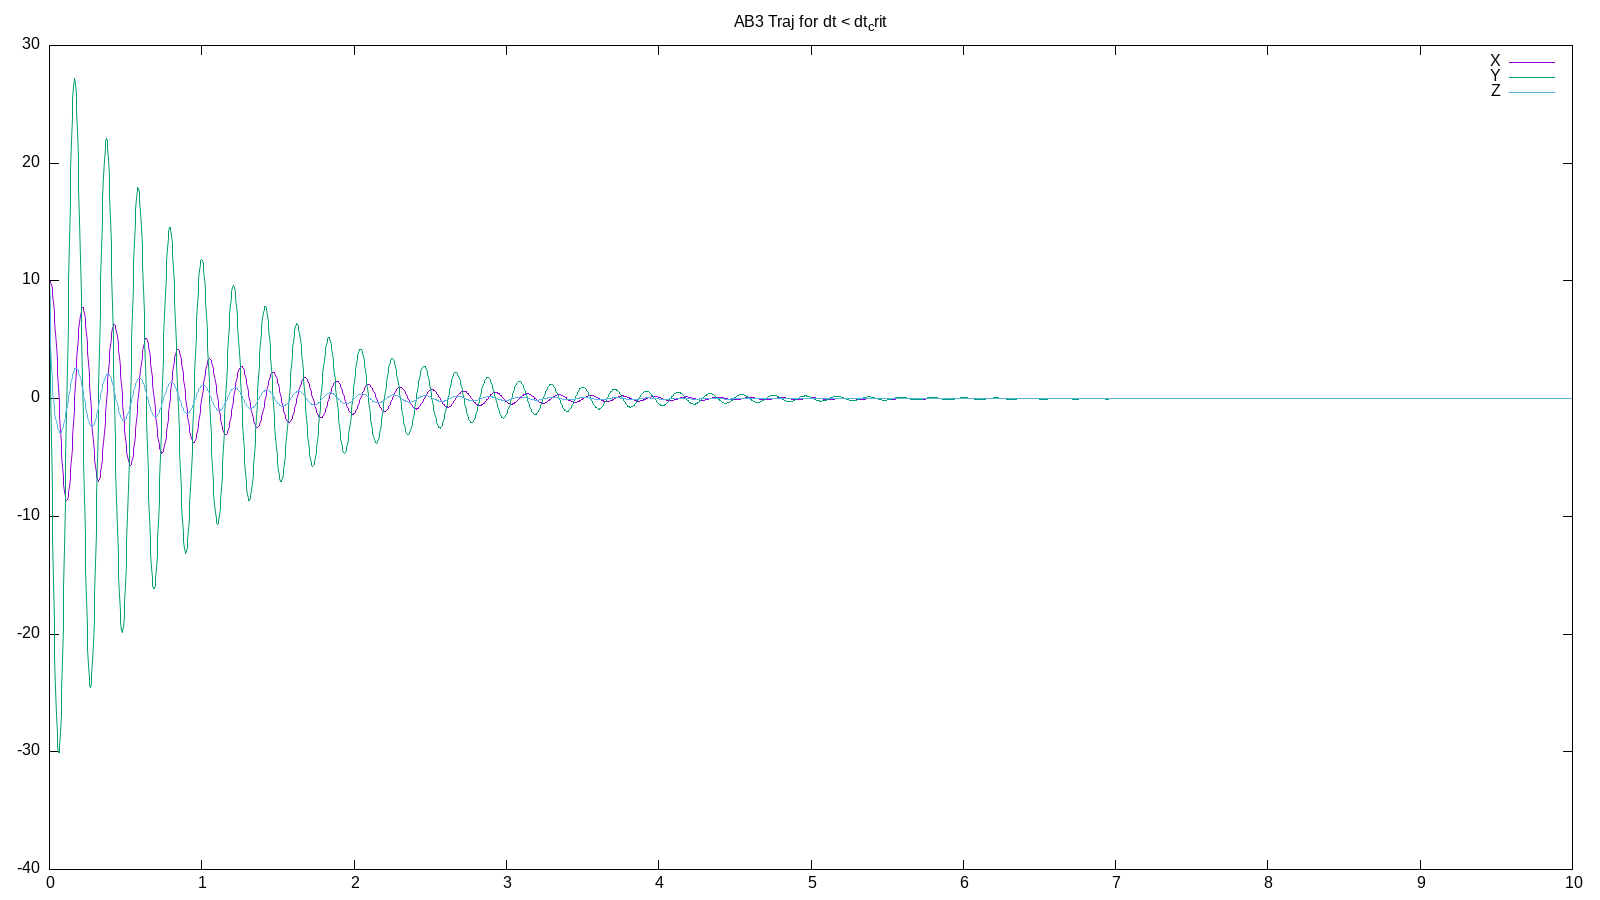
\includegraphics[width=1\textwidth]{1cdt<dt_crit.png}
    \end{minipage}

    \begin{minipage}{0.6\textwidth}
        \centering
        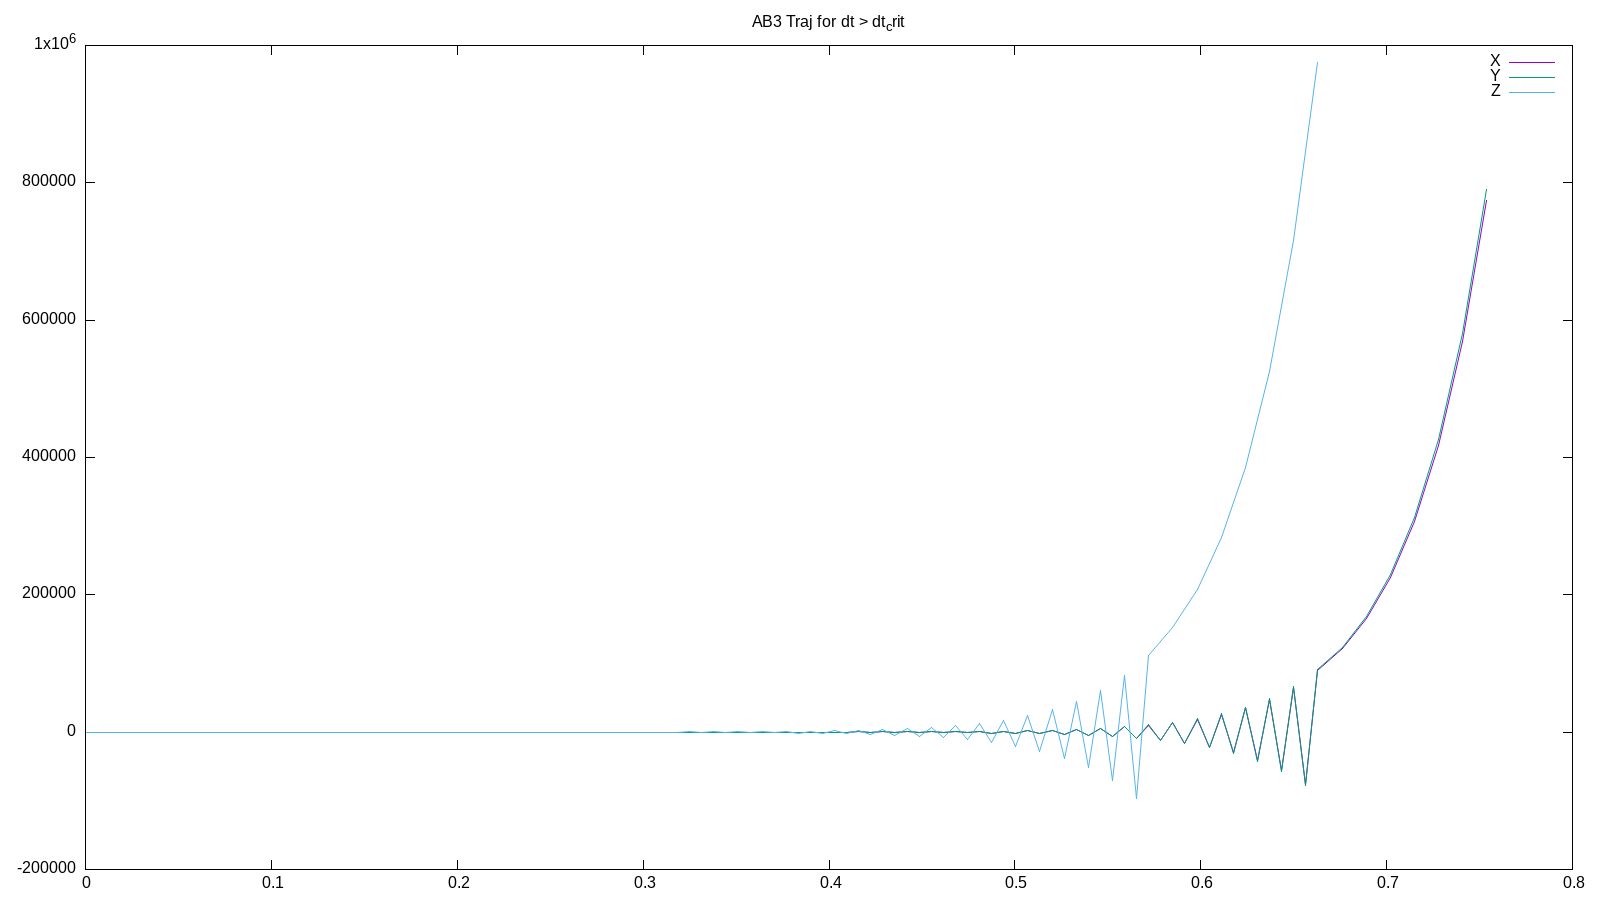
\includegraphics[width=1\textwidth]{1cdt>dt_crit.png}
    \end{minipage}
    \caption{Plots of AB3 with distinct $\dt$. (Top-left: $\dt = 10^{-4}$, 
    Top-right: $\dt = \dt^* - 10^{-4}$, Bottom: $\dt = \dt^* +10^{-4}$)}
  \end{figure}

\end{enumerate}


\section*{Question 2: Convergence and Asbolute Stability for the BDF3 Method}

\begin{enumerate}[label=\alph*)]

  \item \hl{Don't forget about this}

  \item No, BDF3 is not A-stable. This is clear from the plot since the region
  of absolute stability intersects the ``imaginary'' (y) axis in the complex
  plane. Because of this, there is some part of $\C^-$ which is not in the
  region of absolute stability. Thus, BDF3 is not A-Stable.

  \begin{figure}[h]
    \centering
    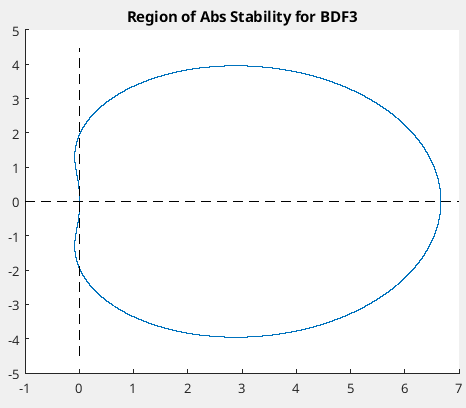
\includegraphics[width=0.6\textwidth]{2bAbsStabReg.png}
    \caption{Region of Abs. Stab. is outside of the plotted boundary}
  \end{figure}

\end{enumerate}

\section*{Question 3: Consistency, Convergence, and Stability for an LMM}

\begin{enumerate}[label=\alph*)]

  \item 
    
  \begin{proof}
    Proving consistency with order two is a mere matter of condidering the
    Taylor Expansion for this LMM. We have by the definition of local truncation
    error, 
    \begin{align}
       \bs{y}_{k+2} - 4\bs{y}_{k+1} + 3\bs{y}_k = -2\dt\bs{f}(\bs{u}_k, t_k) + \dt\tau_{k+2}
    \end{align}
    \begin{align*}
       \bs{y}_{k+2} &= \bs{y}_k + 2\dt \bs{\dot{y}}_k +
       \frac{4\dt^2}{2}\bs{\ddot{y}}_k + \frac{8\dt^3}{6}\bs{\dddot{y}}_k +  h.o.t.\\
       \bs{y}_{k+1} &= \bs{y}_k + \dt \bs{\dot{y}}_k + \frac{\dt^2}{2}\bs{\ddot{y}}_k 
       + \frac{\dt^3}{6}\bs{\dddot{y}}_k +h.o.t. \\
       \dt\tau_{k+2} &=  \bs{y}_k + 2\dt \bs{\dot{y}}_k +
       \frac{4\dt^2}{2}\bs{\ddot{y}}_k + \frac{8\dt^3}{6}\bs{\dddot{y}}_k +
       h.o.t \\ &- 4\left(\bs{y}_k + \dt \bs{\dot{y}}_k + \frac{\dt^2}{2}\bs{\ddot{y}}_k 
       + \frac{\dt^3}{6}\bs{\dddot{y}}_k +h.o.t. \right)\\ &+ 3\bs{y}_k +
       2\dt\bs{f}(\bs{u}_k, t_k)\\
       \tau_{k+2} &=  \frac{4\dt^2}{6}\bs{\dddot{y}}_k, \quad \implies \quad
       |\tau_{k+2}| = \frac{4\dt^2}{6}|\bs{\dddot{y}}_k|
    \end{align*}
    Thus we obtain order 2 convergence for this LMM.
  \end{proof}

  \item 

  \begin{proof}
    Next in order to demonstrate the zero-stability for this LMM we consider the
    root condition for the first characteristic polynomial. We have from this
    LMM, a characteristic polynomial, 
    \begin{align}
        \rho(z) = z^2 - 4z + 3
    \end{align}
    This polynomial has roots $z = 1$ and $z = 3$, the second of which lies
    outside of the unit disk. Therefore this LMM fails the root condition and is
    necessarily zero-unstable. This also implies that this LMM is not convergent
    since congergence is dependent on consistency and zero-stability. 
  \end{proof}

  \item 

  \begin{proof}
    Finally, we can cite the lemma from the notes which states that all
    zero-unstable, consistent LMMs are necessarily unconditionally absolutely
    unstable. We can also look at the region of absolute stability in the figure
    3. This region of absolute stability has no intersection with $\C^-$
    whatsoever. Thus, there is no condition which this LMM is absolutely stable.
    Hence, this LMM is A-unstable. 
    \begin{figure}[h]
        \centering
        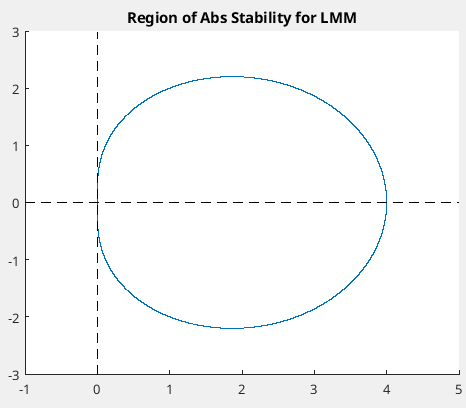
\includegraphics[width=0.6\textwidth]{3cAbsStabRegion.png}
        \caption{Region of Abs. Stab. is inside the boundary}
    \end{figure}

    Note that the region of absolute stability is obtained by plotting,
    \begin{align*}
        \lambda\dt = \frac{e^{i2\theta} - 4e^{i\theta} + 3}{2}
    \end{align*}

  \end{proof}

\end{enumerate}

\section*{Question 4: Convergence and Stability for an RK Method}

\begin{enumerate}[label=\alph*)]
 
 \item

 \begin{proof}
    Proving an explcit RK3 method is convergent requires two things. First, we
    must show that it is consistent, and then that it is zero-stable.
    Zero-stability is implied since all explicit RK methods are necessarily
    one-step methods, i.e. $\rho(z) = z - 1$ which has one simple root $\to$
    satisfies the root condition. Consistency is much more difficult.
    Referencing the notes, we see that there is a well defined criterion for
    explicit RK3 methods to have consistency. We will employ that here. There
    are 4 conditions, 
    \begin{align*}
        b_1 + b_2 + b_3 &= 1, \quad 
        &\frac{2 + 4}{9} + \frac{1}{3} = 1\\
        b_2c_2 + b_3c_3 &= \frac{1}{2}, \quad 
        &\frac{1}{3}\cdot\frac{1}{2} + \frac{4}{9}\cdot\frac{3}{4} = \frac{1}{6} +
        \frac{1}{3} = \frac{1}{2}\\
        b_2c_2^2 + b_3c_3^2 &= \frac{1}{3}, \quad
        &\frac{1}{3}\cdot\frac{1}{4} + \frac{4}{9}\cdot\frac{9}{16} = \frac{1}{12} +
        \frac{1}{4} = \frac{1}{3}\\
        b_3a_{32}c_2 &= \frac{1}{6}, \quad 
        &\frac{4}{9}\cdot\frac{3}{4}\cdot\frac{1}{2} = \frac{1}{6}
    \end{align*}
    They are, so we conclude that since this RK3 method is zero-stable and
    convergent that it is a convergent method. 
 \end{proof}

 \item

 \begin{proof}
    Finally with this RK3 method we will use the standard method for determining
    absolute stability. We look for $|S(z)| < 1$, and for this method to be
    A-stable, we require that this is satisfied for all $z \in \C^-$. To compute
    this, we use the defintion of $S(z)$ from the notes, where $A$ and $b$ are
    parts of the coefficient matrix for this RK3 method, and $h$ is a column
    vector of ones. After plotting the contours of this function on the complex
    plane, we see that the region of absolute stability is small and does not
    contain $\C^-$. This is doubly confirmed by the fact that this method is an
    explicit method, implying that it couldn't be A-stable. 
    \begin{align}
        S(z) = \det(\I - zA + zhb^T)
    \end{align}
    \begin{figure}[h]
        \centering
        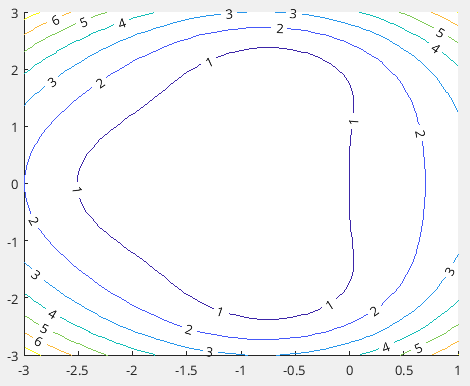
\includegraphics[width=0.6\textwidth]{4cAbsStab.png}
        \caption{Contour Plot of $|S(z)|$ (Region of Abs. Stab. inside
        $|S(z)|$=1 contour)}
    \end{figure}
   
 \end{proof}


\end{enumerate}


\end{document}
